\section{High Level Considerations}

Before diving into the details of consensus mechanisms, let's take a look at the advantages and limitations of using blockchain:

\begin{table}[h]
\begin{tabularx}{\linewidth}{>{\parskip1ex}X@{\kern4\tabcolsep}>{\parskip1ex}X}
\toprule
\hfil\bfseries \color{Orange}{Pros}
&
\hfil\bfseries \color{Orange}{Cons}
\\\cmidrule(r{3\tabcolsep}){1-1}\cmidrule(l{-\tabcolsep}){2-2}

%% PROS
Among the main benefits, \textbf{\color{Blue}{decentralization}} emerges as one of the key pillars, enabling a distributed network in which no central authority has absolute control. This not only increases the security and reliability of the network, but also promotes \textbf{\color{Blue}{transparency and trust}} among participants, making every transaction traceable and verifiable by anyone. In addition, the \textbf{\color{Blue}{immutability}} of data recorded on the blockchain, coupled with its \textbf{\color{Blue}{high availability}}, ensures that information is protected from manipulation and \textbf{\color{Blue}{always accessible}} when needed. These benefits, along with process simplification, efficiency in regulations and \textbf{\color{Blue}{cost savings}}, turn blockchain into a \textbf{\color{Blue}{reliable and programmable platform}} for a wide range of applications. Specifically, cost savings result from the elimination of intermediaries in transactions, enabling a direct transfer of value between the parties involved.
&

%% CONS
However, despite its advantages, blockchain technology also has some significant limitations that hinder its wider adoption. The appearance of the \textbf{\color{Blue}{new technology}}, for example, poses challenges in terms of familiarization and implementation for many organizations. In addition, the \textbf{\color{Blue}{scalability}} of blockchain, especially in public networks, may be limited with respect to the needs of high-frequency transactions. The issue of data \textbf{\color{Blue}{privacy and confidentiality}} remains an area of concern, as information recorded on the blockchain is permanent and accessible to all participants. \textbf{\color{Blue}{Limited adoption}}, \textbf{\color{Blue}{interoperability}} between different blockchain platforms, and complex \textbf{\color{Blue}{regulatory issues}} represent additional challenges that must be overcome to maximize the potential of blockchain technology.
\\\bottomrule
\end{tabularx}
\caption{Benefits and Limitations of Blockchain Technology}
\end{table}

\section{DLT Categories}
\textbf{Distributed Ledger Technologies} (DLTs) can be categorized in different ways based on their use and structure. One of the main categories is Blockchain, which is a specific type of DLT used for shared and immutable ledgers.

Blockchain can be further divided into three main types: public, private and consortium. \textbf{\textcolor{Blue}{Public blockchains}} are open to anyone who wants to participate and are decentralized. \textbf{\textcolor{Blue}{Private blockchains}} are controlled by a centralized organization or entity and are accessible only to authorized users. \textbf{\textcolor{Blue}{Consortial blockchains}} are managed by a group of organizations working together to manage the network.

In addition to blockchains, there are other types of DLTs such as Sidechains and Distributed Ledgers. \textbf{\textcolor{Blue}{Sidechains}} are blockchains linked to a main blockchain and can be used for specific purposes or to enhance the functionality (scalability) of the main blockchain. \textbf{\textcolor{Blue}{Distributed Ledgers}}, on the other hand, are shared ledgers that can be customized for specific purposes and are not necessarily blockchain-based.

\begin{figure}[h]
\centering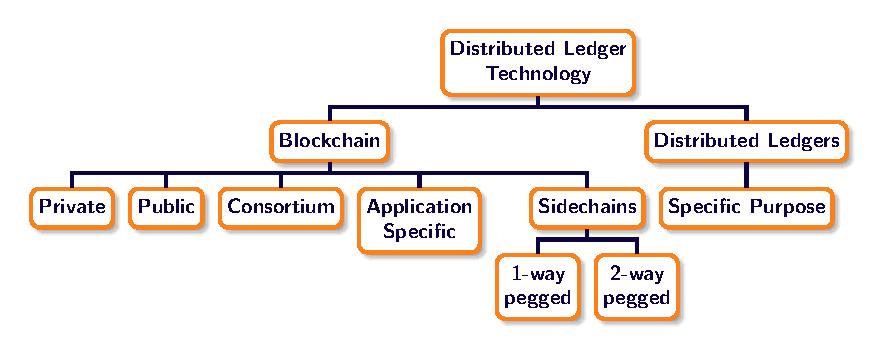
\includegraphics[scale=1]{tikz/chapter3 - DLT.pdf}
\caption{Distributed Ledger Technologies Categories}
\end{figure}

\section{Byzantine Generals Problems}
The Byzantine Generals problem is a fundamental concept in the context of distributed consensus mechanisms. Imagine a situation in which several commanders of an army must coordinate to attack or retreat, but some of them may be traitors or communications between them may be compromised. In this scenario, it is essential that the generals reach a consensus on the strategy to be adopted despite the uncertainty and the presence of potential mistakes or sabotage.

PBFT (Practical Byzantine Fault Tolerance) solves this problem by establishing a set of requirements to ensure reliable consensus among participants (Of course, we are no longer talking about battles, but about blockchain!). These requirements include:
\begin{itemize}
    \item \textbf{Agreement}: All nodes must agree on a single value proposition or decision.
    \item \textbf{Integrity}: Information and transactions must be authentic and unchanged during the consensus process.
    \item \textbf{Validity}: Only valid and legitimate transactions must be accepted and confirmed.
    \item \textbf{Fault Tolerance}: The system must be able to function properly even if some nodes fail or misbehave.
    \item \textbf{Termination}: The consensus process must eventually reach a conclusion and produce a final outcome.
\end{itemize}
Using PBFT, participants can collaborate safely and reliably even in the presence of faulty or malicious nodes. This consensus mechanism is critical to ensuring the consistency and reliability of transactions within distributed networks, such as those based on blockchain technology.

\vspace{2cm}
\section{Security Mechanisms}
In the blockchain, the application of security mechanisms is critical to ensure the security and integrity of transactions. These functions are used in different contexts, below we make a list and it is likely that you already know how some of them work.

\begin{remark}
\textbf{Cryptographic Hash Functions}:
Hash functions are fundamental in the blockchain and are used to confirm and validate new blocks of transactions, to create unique addresses for accounts on the blockchain, to verify the authenticity of messages sent over the network and in Merkle trees.
\end{remark}

\begin{remark2}
\textbf{Asymmetric cryptography}:
A cryptographic technique involving two keys: public and private. 
In the encryption process, the sender encrypts the message with the recipient's public key and, in the case of digital signatures, signs the message with his own private key, while the recipient verifies the signature using the sender's public key.
\end{remark2}

\begin{remark}
\textbf{Merkle trees}:
A data structure that ensures the integrity of transactions in the blockchain.
Transactions are organized in a binary tree, and hashes are used to ensure the integrity of the structure.
They allow for quick verification of whether a transaction is included in a blockchain without having to examine all transactions.
\end{remark}


\section{Type of Consensus Mechanisms}
When it comes to exploring the vast world of consensus mechanisms within blockchains, we are faced with a myriad of options. However, we will focus mainly on three of them: the Proof of Work, the Proof of Stake and the Delegated Proof of Stake. 

\faBitcoin \quad \textbf{Proof of Work} (PoW):

In PoW, participants, called "miners," compete to solve complex cryptographic puzzles.
The first miner to solve the puzzle gains the right to create and confirm a new block of transactions on the blockchain.
This process requires an enormous amount of computing power, making the system secure but also energy intensive.

\faEthereum \quad \textbf{Proof of Stake} (PoS):

In PoS, the right to create and validate a new block depends on the amount of cryptocurrency owned and "played" by participants, called "validators."
The more cryptocurrency that is "played," the greater the probability of being chosen to validate a block and receive rewards.
Because it does not require as intensive computing power as PoW, PoS is more energy efficient.

\faUsers \quad \textbf{Delegated Proof of Stake} (DPoS):

In DPoS, participants elect "delegates" responsible for creating and confirming blocks.
These delegates are voted on by other participants based on trust and reputation.
DPoS is designed to scale more efficiently than PoW and PoS, allowing for faster confirmation of transactions. 

\section{Blockchain Trilemma}


The trilemma of \textbf{decentralization}, \textbf{scalability} and \textbf{security} is one of the most significant challenges in designing and implementing an effective blockchain. The consensus mechanism plays a crucial role in balancing these three dimensions.

\begin{figure}[!htbp]
\centering
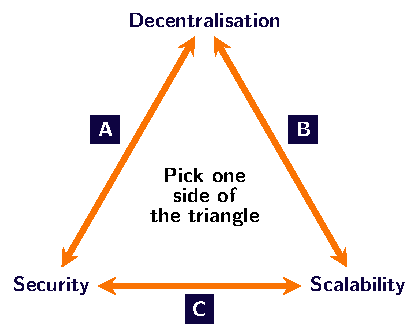
\includegraphics[width=0.6\linewidth]{tikz/chapter3 - Trilemma.pdf}
\caption{The Blockchain Trilemma}
\end{figure}

\textbf{\textcolor{Orange}{Decentralisation}} refers to the \textbf{distribution of decision-making power} among network participants rather than concentrating it in a single centralized entity. An effective consensus mechanism should ensure that no single actor or group of actors has complete control over the network, thus promoting decentralization. However, decentralization can be challenged by the need to reach agreement on transactions and state updates among geographically distributed nodes.

\textbf{\textcolor{Orange}{Scalability}} refers to the \textbf{ability of the system to handle an increasing number of transactions} and to grow efficiently as the workload increases. An efficient consensus mechanism should enable the network to process a large number of transactions quickly and economically without compromising its security or decentralization. However, achieving scalability can be hampered by the computational complexity and communication required to achieve distributed consensus.

\textbf{\textcolor{Orange}{Security} is critical} to \textbf{protect the network from malicious attacks, manipulation, and fraud}. A robust consensus mechanism should ensure the integrity and immutability of data stored on the blockchain, as well as resistance to attack attempts by malicious actors. However, maintaining a high level of security may require compromises on the speed or scalability of the network.

To address the trilemma, there are two main approaches in designing consensus mechanisms:
\begin{itemize}
    \item \textbf{Message-based consensus mechanisms}: in this approach, network participants communicate with each other to reach consensus on the validity of transactions and the state of the blockchain. 
    \item \textbf{Shared memory-based consensus mechanisms}: in this approach, participants share a common memory space and use synchronization techniques to ensure that all nodes in the network agree on the state of the system. 
\end{itemize}

\section{Distributed Consensus}
In the context of distributed systems, reaching consensus among nodes that do not trust each other on the final state of data is of paramount importance. This process ensures that all nodes within the network agree on the validity and order of transactions. Several algorithms are employed to accomplish this task, falling primarily into two categories:

\textbf{\textcolor{Blue}{Approaches Based on Proof and Leader Election by Lottery}}: These consensus mechanisms rely on cryptographic proof or random selection of leaders to propose and validate transactions. An example of this category is Proof of Work (PoW), where nodes compete to solve cryptographic puzzles in order to validate transactions and add blocks to the blockchain.

\textbf{\textcolor{Blue}{Based on Byzantine Failure Tolerance (BFT)}}: These approaches focus on the ability to resist failures and malicious actions within the system. A notable example is Practical Byzantine Fault Tolerance (PBFT), which involves a consensus process among a select group of nodes that must be at least a majority to ensure the integrity of the system.

Let us now look at some key aspects related to Distributed Consensus:

\faBug \quad \textbf{Failure Tolerance and Replication}

Failure tolerance is critical in a distributed environment because it implies the \textbf{ability of the system to continue to function} even in the presence of malfunctions or failures. Inevitably, any system can incur problems, and the distributed system is no exception. Replication is an effective strategy for dealing with problems related to failing nodes. It replicates the behavior of nodes so that, should one or more nodes fail or behave non-compliantly, the system can still operate consistently.

\textbf{Machine State Replication} is a technique that aims to ensure that all servers have a consistent and identical view of data state. This is achieved by ensuring that all servers start from the same initial state, receive requests in a specific order, and produce the same deterministic output for the same input. This replication process ensures consistency and uniformity across the system, regardless of the condition of each node.

\faLock \quad \textbf{Lower Limits and Security}

When dealing with Distributed Consent, it is important to understand the lower limits necessary to ensure that the system works properly. These limits are defined in terms of the \textbf{number of nodes required to achieve consensus}. In the case of Classical Federated Consensus (CFT), at least \texttt{2F + 1} nodes are required to ensure consensus, while in the case of Byzantine Failure Tolerance (BFT), at least \texttt{3F + 1} nodes are required. These minimum requirements are essential to ensure that the system is protected from malicious attacks or accidental failure.

N.B. "\texttt{F}" represents the maximum number of nodes that can fail within a distributed system without compromising its integrity or ability to achieve consensus.

In addition, for the consensus process to be considered valid and reliable, transactions \textbf{must meet certain security and functionality requirements}. These include agreement on an end state of the data, integrity of the transactions, their validity against the rules of the protocol, and the defined and stable conclusion of the consensus process. 

\section{Distributed Consensus Protocols}
Here are some very different approaches to achieving consensus within a distributed network.

\colorbox{Orange!70}{\textbf{\makebox(100,7){Paxos (Lamport)}}}
\vspace{-0.3cm}
\begin{itemize}
    \item Uses \texttt{2F + 1} processes to ensure failure tolerance.
    \item It is based on a two-stage protocol: the \textbf{preparation stage} and the \textbf{acceptance stage}.
    \item Participants include \textbf{proposers}, who propose values, and \textbf{acceptors}, who accept the proposed values.
\end{itemize}


\colorbox{Orange!70}{\textbf{\makebox(165,7){Raft (Ongaro \& Ousterhout)}}}
\vspace{-0.3cm}
\begin{itemize}
    \item Assumes that the \textbf{leader is always honest}.
    \item Elects a single leader in each "term" (unit of time).
    \item Solves three main problems: leader election, log replication, and security.
\end{itemize}

\colorbox{Orange!70}{\textbf{\makebox(250,7){Practical Byzantine Fault Tolerance (PBFT)}}}
\vspace{-0.3cm}
\begin{itemize}
    \item It consists of three sub-protocols: \textbf{normal operation}, \textbf{view change} and \textbf{checkpoint}.
    \item It divides operations into \textbf{pre-preparation}, \textbf{preparation} and \textbf{confirmation phases}.
    \item The participants are \textbf{replicas}, with one of them designated as the primary node and the others as backups.
    \item It ensures Byzantine failure tolerance with a number of nodes \texttt{N $\geq$ 3F + 1}.
    \item Uses digital signatures and certificates to maintain the integrity of operations.
    \item The \textbf{view-change protocol} is triggered when the primary node is suspected of being faulty.
    \item The \textbf{checkpoint sub-protocol} discards old messages in replica logs to ensure data consistency.
\end{itemize}

Paxos, Raft, and PBFT are distributed consensus protocols with specific features and mechanisms to ensure fault tolerance and secure operations. However, let us now look in detail at the alternatives that are most popular today, namely Proof of Work (PoW) and Proof of Stake (PoS).

\section{Proof of Work (PoW)}
\colorbox{Orange!70}{\textbf{\makebox(125,7){Proof of Work (PoW)}}} works through a competitive process in which miners compete to solve complex mathematical problems. \textit{But how does it work practically?}

Basically, a node proposing a block must find a "nonce" (a random number) such that the \textbf{hash of the block}, together with the nonce, is \textbf{less than a threshold value}. This process requires considerable computational effort. Miners search for the nonce through trial and error, varying the nonce until they find a value that meets the difficulty requirement. Once found, the proposed block is inserted in the network and \textbf{nodes check the validity} of the block and add it to the chain.

Hence, PoW has some important properties, which we list below:
\begin{itemize}
    \item \textbf{\textcolor{Blue}{Common Prefix Property}}: Ensures that honest nodes share a large common prefix in the blockchain. If this is not done, agreement between nodes on the same chain cannot be guaranteed, compromising the security of the network.
    \item \textbf{\textcolor{Blue}{Chain Quality Property}}: Ensures that the blockchain contains a minimum level of correct blocks created by honest nodes. If this chain quality is compromised, the validity of the chain itself cannot be guaranteed, opening up the possibility of security breaches.
    \item \textbf{\textcolor{Blue}{Chain Growth Property}}: Implies that new correct blocks are continuously added to the blockchain. If chain growth is affected, the network's ability to maintain its uptime (liveness) can be compromised, potentially causing blockages or system paralysis.
\end{itemize}
    
Furthermore, \textbf{target difficulty} is an essential parameter in the context of the Bitcoin protocol. It is a fundamental value that is regularly updated every 2016 blocks, ensuring a stable block creation rate of approximately 10 minutes. It represents the \textbf{maximum value a block hash must have} to be considered valid.

\textbf{Incentives} also play a vital role in this case. In the case of Bitcoin, miners are rewarded with a per block reward and transaction fees. These economic incentives \textbf{motivate miners to continue participating in the mining process}, ensuring the security and stability of the network.

\section{Proof of Stake (PoS)}
\colorbox{Orange!70}{\textbf{\makebox(120,7){Proof of Stake (PoS)}}} is a consensus algorithm used in blockchain that differs significantly from Proof of Work (PoW). In PoS, there is no traditional concept of "mining" as in PoW, where miners compete to solve complex mathematical problems. Instead, PoS participants are called validators or stakeholders and \textbf{participate in the consensus process by putting a portion of their cryptocurrency}, known as a "stake," into play.

Variants of PoS include \textbf{Chain-based PoS}, \textbf{Committee-based PoS} and \textbf{Delegated PoS}, each with its own characteristics and consensus mechanisms. For example, in Chain-based PoS, blocks are validated based on the number of coins owned by the participant, while in Committee-based PoS, a selected committee validates blocks based on specific rules. Delegated PoS allows participants to delegate their stake to a trusted node that acts as a validator on their behalf.

The process of earning rewards in PoS is sometimes called "virtual mining" because participants do not have to solve complex mathematical puzzles, but instead \textbf{must prove that they own a significant amount of cryptocurrency} and contribute to the security and validity of the network. Control over the majority of the network also remains crucial in PoS, as control over a large amount of stakes allows a single actor to influence consensus decisions and potentially attack or control the network.



